
\section{The Fitting Method}
\label{dga:sec:fitting}

Our fitting method uses the abundances of an ensemble of stars, incorporating
age measurements as additional data where available, and without any binning,
accurately constructs the~\textit{likelihood function}
$L(\script{D} | \{\theta\})$ describing the probabiliy of observing the
data~$\script{D}$ given a set of model parameters $\{\theta\}$.
$L(\script{D} | \{\theta\})$ is related to the~\textit{posterior probability}
$\L(\{\theta\} | \script{D})$ according to Bayes' Theorem:
\begin{equation}
L(\{\theta\} | \script{D}) = \frac{
	L(\script{D} | \{\theta\}) L(\{\theta\})
}{
	L(\script{D})
},
\label{dga:eq:bayes}
\end{equation}
where~$L(\{\theta\})$ is the likelihood of the parameters themselves (known as
the~\textit{prior}) and~$L(\script{D})$ is the likelihood of the data (known as
the~\textit{evidence}).
Although it is more desirable to measure the posterior probability, in practice
only the likelihood function can be robustly determined because the prior is
not directly quantifiable.
The prior requires quantitative information independent of the data on the
accuracy of a chosen set of parameters~$\{\theta\}$.
With no additional information on what the parameters should be, the best
practice is to assume a ``flat'' or ``uniform'' prior in which~$L(\{\theta\})$
is a constant, and therefore~$L(\{\theta\} | \script{D}) \approx
L(\script{D} | \{\theta\})$; we retain this convention here unless otherwise
stated.
\par
As mentioned in~\S~\ref{dga:sec:intro}, the sampling of stars from an underlying
evolutionary track in abundance space proceeds according to an IPPP
\citep[e.g.,][]{Press2007}.
Due to its detailed nature, we reserve a full derivation of our likelihood
function for Appendix~\ref{dga:sec:likelihood} and provide qualitative discussion
of its form here.
Though our use case in the present paper is in the context of one-zone GCE
models, our derivation assumes only that the chief prediction of the model is
a track of some arbitrary form in the observed space.
It is therefore highly generic and should be easily extensible to other
astrophysical models that predict tracks of some form (e.g., stellar streams
in kinematic space and stellar isochrones on CMDs).
\par
In practice, the evolutionary track predicted by a one-zone GCE model is
generally not known in some analytic functional form (unless specific
approximations are made as in, e.g.,~\citealp{Weinberg2017b}).
Instead, it is most often quantified as a piece-wise linear form predicted by
some numerical code (in our case,~\vice).
For a sample~$\script{D} = \{\script{D}_1, \script{D}_2, \script{D}_3, ...,
\script{D}_N\}$ containing~$N$ abundance and age (where available) measurements
of individual stars and a track~$\script{M} = \{\script{M}_1, \script{M}_2,
\script{M}_3, ..., \script{M}_K\}$ sampled at~$K$ points in abundance space,
the likelihood function is given by
\begin{equation}
\ln L(\script{D} | \{\theta\}) = \sum_i^N \ln \left(
\sum_j^K w_j \exp\left(
\frac{-1}{2}\Delta_{ij}C_i^{-1}\Delta_{ij}^T
\right)
\right),
\label{dga:eq:likelihood}
\end{equation}
where~$\Delta_{ij} = \script{D}_i - \script{M}_j$ is the vector difference
between the~$i$th datum and the~$j$th point on the predicted track,~$C_i^{-1}$
is the inverse covariance matrix of the~$i$th datum, and~$w_j$ is a weight to
be attached to~$\script{M}_j$ (we clarify our notation that~$ij$ refers to a
data-model pair and not a matrix element; the covariance matrix need not be
diagonal for this approach).
This functional form is appropriate for GCE models in which the normalization
of the SFH is inconsequential to the evolution of the abundances; in the
opposing case where the normalization does impact the predicted abundances,
one additional term subtracting the sum of the weights is required (see
discussion below).
\par
Equation~\refp{dga:eq:likelihood} arises from marginalizing the likelihood of
observing each datum over the entire evolutionary track and has the more
general form of
\begin{subequations}\begin{align}
\ln L(\script{D} | \{\theta\}) &= \sum_i^N \left(
\int_\script{M} L(\script{D}_i | \script{M}) d\script{M}
\right)
\label{dga:eq:likelihood_general_int}
\\
&\approx \sum_i^N \ln \left(
\sum_j^K L(\script{D}_i | \script{M}_j)\right).
\label{dga:eq:likelihood_general}
\end{align}\end{subequations}
Equation~\refp{dga:eq:likelihood_general} follows from equation
\refp{dga:eq:likelihood_general_int} when the track is densely sampled by the
numerical integrator (see discussion below), and equation~\refp{dga:eq:likelihood}
follows thereafter when the likelihood $L(\script{D}_i | \script{M}_j)$ of
observing the~$i$'th datum given the~$j$th point on the evolutionary track is
given by a weighted~$e^{-\chi^2/2}$ expression.
Mathematically, the requirement for this marginalization arises naturally from
the application of statistical likelihood and an IPPP to an evolutionary track
(see Appendix~\ref{dga:sec:likelihood}).
Qualitatively, this requirement is due to observational uncertainties -- there
is no way of knowing which point on the evolutionary track the
datum~$\script{D}_i$ is truly associated with, and the only way to properly
account for its unknown position is to consider all pair-wise combinations
of~\script{D}~and~\script{M}.
\par
The mathematical requirement for a weighted as opposed to unweighted
$e^{-\chi^2/2}$ likelihood expression also arises naturally in our derivation.
Qualitatively, the weights arise because the likelihood of observing the datum
$\script{D}_i$ is proportionally higher for points on the evolutionary track
when the SFR is high or if the survey selection function is deeper.
For a selection function~\script{S}~and SFR~$\dot{M}_\star$, the weights should
scale as their product:
\begin{equation}
w_j \propto \script{S}(\script{M}_j | \{\theta\})
\dot{M}_\star(\script{M}_j | \{\theta\}).
\label{dga:eq:weights}
\end{equation}
Whether or not the weights require an overall normalization is related to the
parametrization of the GCE model -- in particular, if the normalization of the
SFH impacts the abundances or not (see discussion below).
The selection function may be difficult to quantify, but one simple way to
characterize its form in chemical space would be to assess what fraction -- by
number -- of the stellar populations in the model would be incorporated into
the sample as a result of cuts in, e.g., color, surface gravity, effective
temperature, etc.
\par
The marginalization over the track and the weighted likelihood are of the
utmost importance to ensure accurate best-fit parameters.
In our tests against mock samples (see~\S~\ref{dga:sec:mocks} below), we are unable
to recover the known evolutionary parameters of input models with discrepancies
at the many-$\sigma$ level if either are neglected.
While these details always remain a part of the likelihood function, equation
\refp{dga:eq:likelihood} can change in form slightly if any one of a handful of
conditions are not met.
We discuss these conditions and the necessary modifications below, referring to
Appendix~\ref{dga:sec:likelihood} for mathematical justification.
\par
\textit{The model track is infinitely thin.}
In the absence of measurement uncertainties, all of the data would fall
perfectly on a line in the observed space.
As discussed in the beginning of~\S~\ref{dga:sec:onezone}, the fundamental
assumption of one-zone GCE models is instantaneous mixing of the various
nuclear species throughout the star forming reservoir.
Consequently, the ISM is chemically homogeneous and the model predicts a single
exact abundance for each element or isotope at any given time.
If the model in question instead predicts a track of some finite width, then
the likelihood function will have a different form requiring at least one
additional integral.
\par
\textit{Each observation is independent.}
When this condition is met, the total likelihood of observing the
data~\script{D}~can be expressed as the product of the likelihood of observing
each individual datum:
\begin{subequations}\begin{align}
L(\script{D} | \{\theta\}) &= \prod_i^N L(\script{D}_i | \script{M})
\\
\implies \ln L(\script{D} | \{\theta\}) &= \sum_i^N \ln
L(\script{D}_i | \script{M}).
\end{align}\end{subequations}
This condition plays an integral role in giving rise to the functional form of
equation~\refp{dga:eq:likelihood}, and if violated, the likelihood function will
also have a fundamentally different form.
\par
\textit{The observational uncertainties are described by a multivariate
Gaussian.}
If this condition fails, the weighted~$\chi^2 = \Delta_{ij}C_i^{-1}\Delta_{ij}^T$
expression is no longer an accurate parametrization of~$L(\script{D}_i |
\script{M}_j)$ and it should be replaced with the more general form of
equation~\refp{dga:eq:likelihood_general}.
In these cases, a common alternative would be to replace~$e^{-\chi^2 / 2}$ with
some kernel density estimate of the uncertainty at the point~$\script{M}_j$
while retaining the weight~$w_j$, but this substitution is only necessary for
the subset of~\script{D}~whose uncertainties are not adequately described by a
multivariate Gaussian.
\par
\textit{The track is densely sampled.}
That is, the spacing between the points on the track~\script{M}~is small
compared to the observational uncertainties in the data.
This assumption can be relaxed at the expense of including an additional
correction factor~$\beta_{ij}$ given by equation~\refp{dga:eq:corrective_beta}
that integrates the likelihood between each pair of adjacent
points~$\script{M}_j$ and~$\script{M}_{j + 1}$ along the track (see discussion
in Appendix~\ref{dga:sec:likelihood}).
If computing the evolutionary track is sufficiently expensive, relaxing the
number of points and including this correction factor may be the more
computationally efficient option.
\par
\textit{The normalization of the SFH does not impact the predicted abundances.}
Only the time-dependence of the SFH impacts the abundance evolution predicted
by the GCE model.
As mentioned above, the model-predicted SFH and the selection function of the
survey determine the weights to attach to each point~$\script{M}_j$ along the
track, and if the normalization of the SFH does not impact the abundance
evolution, then it must not impact the inferred likelihood either.
In our detailed derivation of equation~\refp{dga:eq:likelihood}, we find that the
proper manner in which to assign the weights is to normalize then such that
they add up to 1 (see Appendix~\ref{dga:sec:likelihood}).
Some GCE models, however, are parametrized such that the normalization of the
SFH~\textit{does} impact the abundance evolution.
One such example would be if the SFE timescale~$\tau_\star$ (see equation
\ref{dga:eq:taustar} and discussion in~\S~\ref{dga:sec:onezone}) depends on the gas
supply~$M_\text{g}$ in order to implement some version of a non-linear
Kennicutt-Schmidt relation\footnote{
	$\dot{\Sigma}_\star \propto \Sigma_\text{g}^N \implies \tau_\star \propto
	\Sigma_\text{g}^{1 - N}$ where~$N \neq 1$.
	\citet{Kennicutt1998} measured~$N = 1.4 \pm 0.15$ from the global gas
	densities and SFRs in star-forming spiral galaxies, although recent
	advancements suggest more sophisticated forms (e.g.,~\citealp{Krumholz2018b};
	see discussion in~\S~2.6 of~\citealt{Johnson2021}).
} where the normalization of the SFH and size of the galaxy are taken into
account.
In these cases, the likelihood function is given by
equation~\refp{dga:eq:corrective_beta} where the weights remain un-normalized and
their sum must be subtracted from equation~\refp{dga:eq:likelihood}.
This requirement can be qualitatively understood as a penalty for models that
predict data in regions of the observed space where there are none -- a term
which encourages parsimony, rewarding parameter choices which explain the data
in as few predicted instances as possible.
This penalty is still included in models which normalize the weights, with the
tracks that extend too far in abundance space instead having a higher
\textit{fractional} weight from data at large~$\chi^2$, lowering the total
likelihood (see discussion near the end of Appendix~\ref{dga:sec:likelihood}).

% fig 1
\afterpage{
\clearpage
\begin{landscape}
\begin{figure*}
\centering
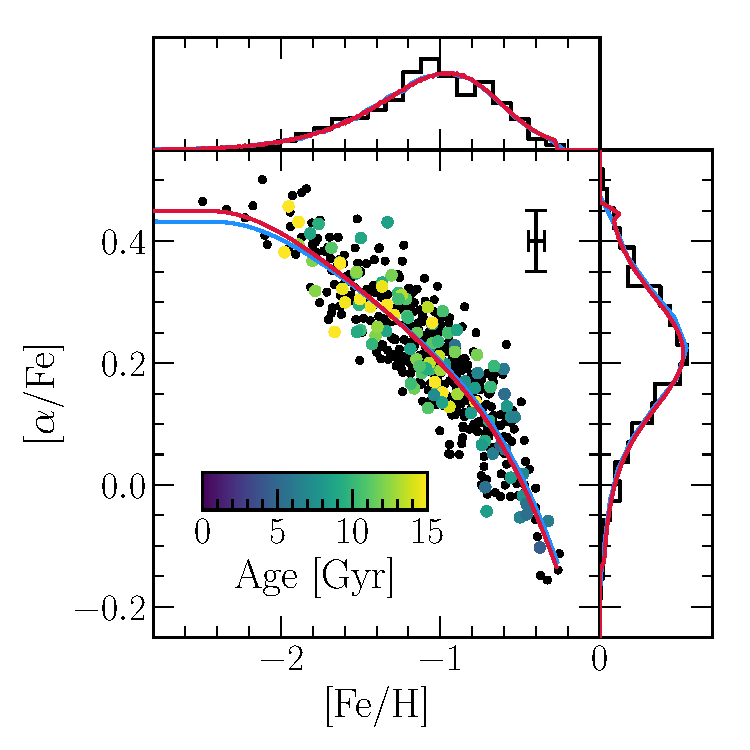
\includegraphics[scale = 0.56]{fiducial_mock_afe_feh.pdf}
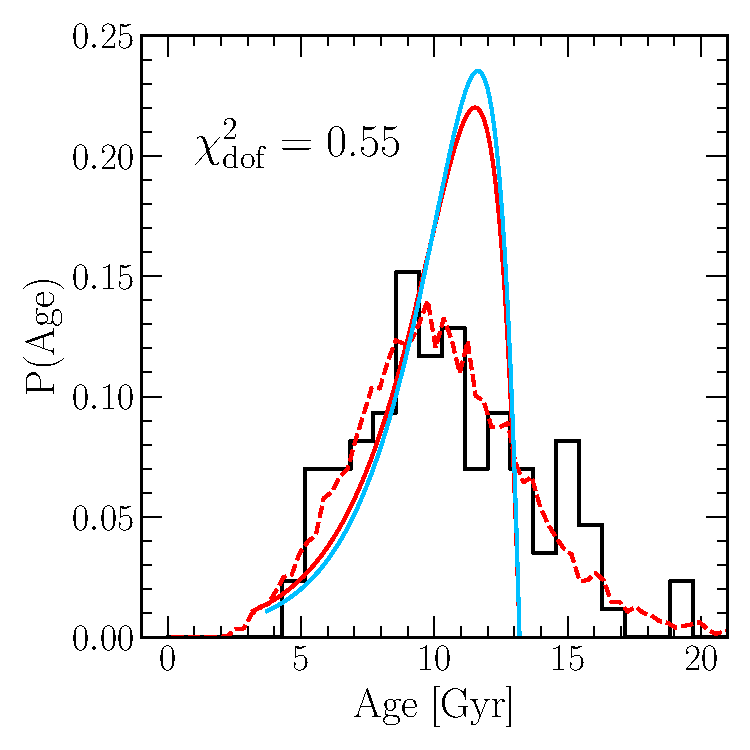
\includegraphics[scale = 0.47]{fiducial_mock_agedist.pdf}
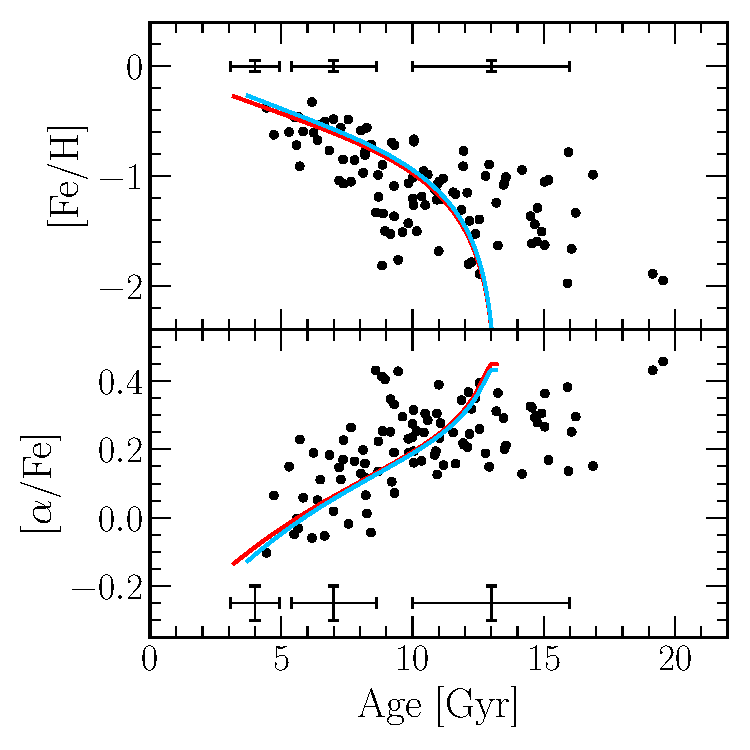
\includegraphics[scale = 0.46]{fiducial_mock_amr.pdf}
\caption{
Our fiducial mock sample.
Red lines in all panels denote the input model while blue lines denote the
recovered best-fit model.
The mock sample has~$N = 500$ stars with abundance uncertainties of
$\sigma_\feh = \sigma_\afe = 0.05$ (marked by the errorbar in the left panel).
$N = 100$ of the stars have age information as indicated by the colourbar in
the left panel with an artificial uncertainty
of~$\sigma_{\log_{10}(\text{age})} = 0.1$.
\textbf{Left}: The mock sample in chemical space, with the marginalized
distributions in~\feh~and~\afe~shown on the top and right, respectively.
\textbf{Middle}: The age distribution of the mock sample (black, binned).
The dashed red line indicates the age distribution obtained by sampling
$N = 10^4$ rather than~$N = 500$ stars from the input model and assuming the
same age uncertainty.
\textbf{Right}: The age-\feh~(top) and age-\afe~(bottom) relations for the mock
sample.
Uncertainties at various ages are marked by the error bars at the top and
bottom of each panel.
}
\label{dga:fig:fiducial_mock}
\end{figure*}
\end{landscape}
\clearpage
}

We demonstrate the accuracy of our likelihood function in~\S~\ref{dga:sec:mocks}
below by means of tests against mock data samples.
Although our likelihood function does not include a direct fit to the
stellar distributions in age and abundances, weighting the inferred likelihood
by the SFR in the model indeed incorporates this information on how many stars
should form at which ages and abundances.
Our method therefore provides~\textit{implicit} fits to the age and abundance
distributions, even though this information is not directly included in the
likelihood calculation.
\par
There are a variety of ways to construct the likelihood distribution in
parameter space.
In the present paper, we employ the MCMC method, making use of
the~\mc~\python~package~\citep{ForemanMackey2013} to construct our Markov
chains.
Despite being more computationally expensive than other methods (e.g.,
maximum a posteriori estimation), MCMC offers a more generic solution by
sampling tails and multiple modes of the likelihood distribution which could
otherwise be missed or inaccurately characterized by the assumption of
Gaussianity.
Our method should nonetheless be extensible to additional data sets described
by GCE models with different parametrizations as well as different methods of
optimizing the likelihood distribution, such as maximum a posteriori estimates.

